\section{Theorie}
\label{sec:Theorie}
\subsection{Gedämpfte Schwingungen}
\label{sec:Gedämpfte_Schwingungen}

Wird einem System, das aus Kondensator und Spule besteht, Energie zugeführt, so kann
diese Energie im System gespeichert werden, indem sie zwischen der Kapazität $C$
des Kondensators und der Induktivität $L$ der Spule hin und her schwingt. In der
Theorie kann dies verlustfrei geschehen, sodass sich eine ungedämpfte Schwingung
ergibt. In der Praxis ist dies allerdings nicht realisierbar, da jeder Leiter einen
Innenwiderstand besitzt und die Schwingung somit gedämpft wird. Zusätzlich kann auch
ein separater Widerstand $R$ in den Schwingkreis eingebaut werden. Mithilfe der Kirchhoff'schen
Regeln ergibt sich dann für diesen Schaltkreis \ref{fig:RLC}
\begin{equation}
  U_{\text{R}}(t)+U_{\text{C}}(t)+U_{\text{L}}(t)=0 \,.
\end{equation}

\begin{figure}
  \centering
  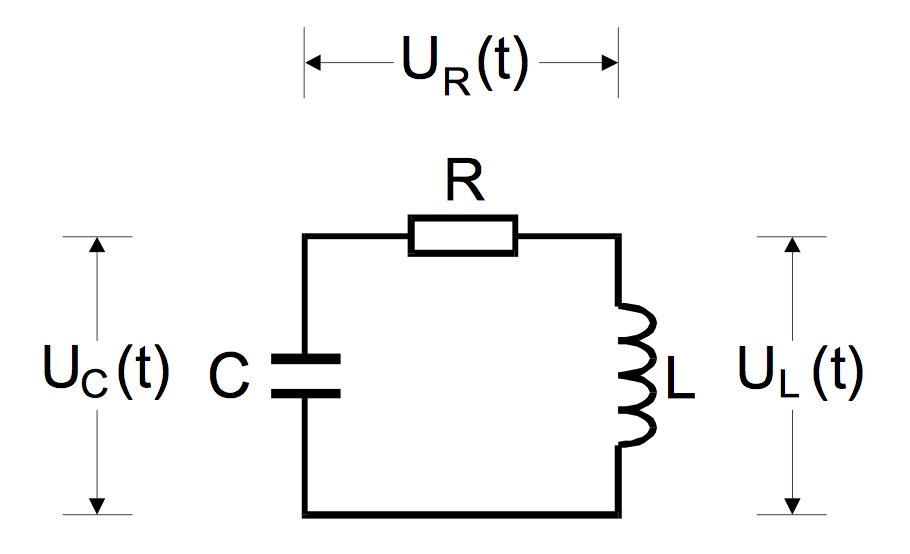
\includegraphics[width=300pt]{data/schwingkreis_theorie.png}
  \caption{Skizze eines RLC Kreises\cite{Versuchsanleitung1}}
  \label{fig:RLC}
\end{figure}
Dabei ist $U_{\text{R}}$ die Spannung am Widerstand, $U_{\text{C}}$ die Spannung
am Kondensator und $U_{\text{L}}$ die Spannung an der Induktivität.
Werden nun die Beziehungen $U_{\text{R}}(t)=R \symbf{I}(t)$,
$U_{\text{C}}(t)=Q(t)/C$ und $U_{\text{L}}(t)=L (\symup{d} \symbf{I}/\symup{d}t)$
eingesetzt und wird nach der Zeit abgeleitet, so ergibt sich die Differentialgleichung
\begin{equation}
  \frac{\symup{d}^2\symbf{I}}{\symup{d}t}+\frac{R}{L}\frac{\symup{d}\symbf{I}}
  {\symup{d}t} + \frac{1}{LC}\symbf{I} = 0
  \label{eqn:DGL}
\end{equation}
für gedämpfte Schwingungen. Zur Lösung kann der Ansatz
\begin{equation}
  \underline{\symbf{I}}(t)\footnote{Komplexe Zahlen werden im Folgenden mit einem
  Unterstrich markiert.}=\underline{U} \exp({i\underline{\omega}t})
  \label{eqn:ansatz}
\end{equation}
gewählt werden. Dann ergibt sich nach Einsetzen von \eqref{eqn:ansatz} in \eqref{eqn:DGL}
der Zusammenhang
\begin{equation}
  \underline{\omega}^2-i\frac{R}{L}\underline{\omega}-\frac{1}{LC}=0 \,.
  \label{eqn:omega}
\end{equation}
Daraus lässt sich die Gesamtlösung der Differentialgleichung \eqref{eqn:DGL} zu
\begin{equation}
  \underline{\symbf{I}}=\exp\biggl(-\frac{R}{2L}t\biggr)\Biggl(\underline
  {U_{\text{1}}}\exp\Biggl(i\sqrt{\frac{1}{LC}-\frac{R^2}{4L^2}}\Biggr)
  +\underline{U_{\symup{2}}}\exp\Biggl(-i\sqrt{
  \frac{1}{LC}-\frac{R^2}{4L^2}}\Biggr)\Biggr)
\end{equation}
bestimmen, indem aus \eqref{eqn:omega} Lösungen für $\underline{\omega}$ bestimmt
und die allgemeine Lösung der Differentialgleichung gemäß des Superpositionsprinzips
gebildet wird. Nun müssen die beiden Fälle
\begin{align}
  \frac{1}{LC}>\frac{R^2}{4L^2} & \qquad\qquad\qquad\text{und} & \frac{1}{LC}<\frac{R^2}{4L^2}
\end{align}
unterschieden werden. Für ersteren ist die Wurzel reell. Damit ergibt sich die
reelle Lösungsfunktion $\symbf{I}$ mit einem geeigeneten Ansatz zu
\begin{equation}
  \symbf{I}=A_{\text{0}}\exp\biggl(-\frac{R}{2L}t\biggr)\cos\Biggl(
  \sqrt{\frac{1}{LC}-\frac{R^2}{4L^2}}t+\eta\Biggr)\,.
\end{equation}
wobei $A_{\text{0}}$ eine beliebige Konstante und $\eta$ eine beliebige Phase ist.
Dies entspricht der GLeichung einer gedämpften Schwingung, da die Amplitude mit zunehmender
Zeit $t$ gegen $0$ geht.
Die für die Abnahmegeschwindigkeit charakteristische Abklingdauer $T_{\text{Ex}}$
wird definiert als
\begin{equation}
  T_{\text{Ex}}\coloneq\frac{2L}{R} \,.
  \label{eqn:abklingdauer}
\end{equation}
Für den zweiten Fall ist die Wurzel imaginär. Dann werden alle Exponentialfunktionen
reell, sodass keine oszillatorischen Anteile mehr vorliegen. Dieser Fall wird
Kriechfall genannt. (...)


Für den Spezialfall
\begin{equation}
  \frac{1}{LC}=\frac{R^2}{4L^2}
\end{equation}
tritt der aperiodische Grenzfall ein. Dies ist die stärkste mögliche Dämpfung eines
Systems.

\subsection{Erzwungene Schwingungen}
\label{Erzwungene_Schwingungen}

An den Schwingkreis wird nun sinusförmige Wechselspannung angelegt. Eine Skizze
hierzu ist in \ref{fig:RLC_sinus} zu finden. Diese hat die Form
\begin{equation}
  \underline{U}(t)=U_{\symup{0}}\exp(i\omega t) \,,
\end{equation}

\begin{figure}
  \centering
  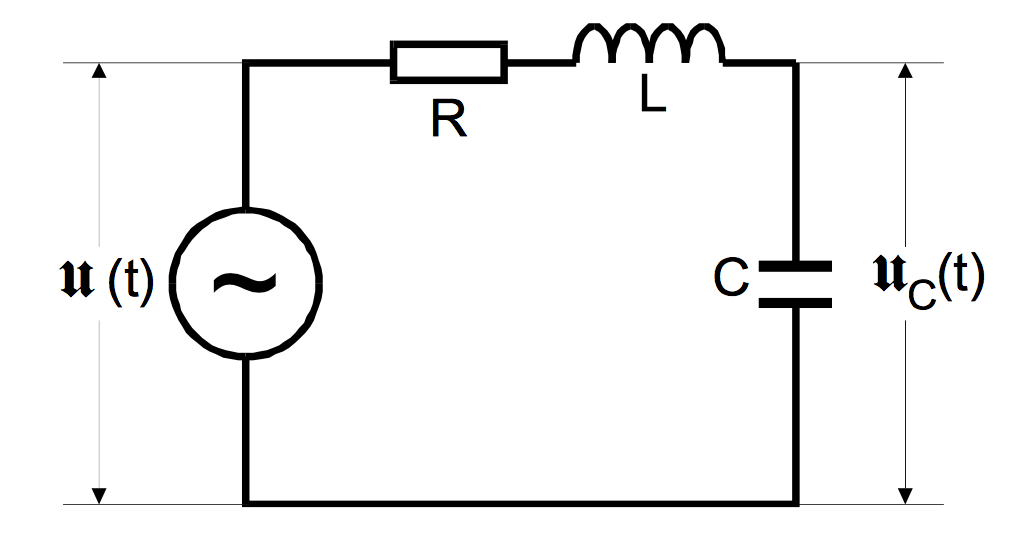
\includegraphics[width=300pt]{data/angeregter_schwingkreis_theorie.png}
  \caption{Skizze eines RLC Kreises mit angelegter sinusförmiger Spannung
  \cite{Versuchsanleitung1}}
  \label{fig:RLC_sinus}
\end{figure}
wodurch die im zuvor diskutierten Fall noch homogene Differentialgleichung zu einer
inhomogenen Differentialgleichung mit der angelegten sinusförmigen Spannung
als Inhomogenität wird:
\begin{equation}
  LC\frac{\symup{d}^2\underline{\symbf{U}}_{\symup{C}}}{\symup{d}t^2}
  +RC\frac{\symup{d}\underline{\symbf{U}}_{\symup{C}}}{\symup{d}t}
  +\underline{\symbf{U}}_{\symup{C}} = U_{\symup{0}}\exp(i\omega t) \,.
\end{equation}
Eine Lösung für diese Differentialgleichung lässt sich mit einem geeigneten Ansatz
zu
\begin{equation}
  -LC\omega^2\underline{U}+i\omega R C\underline{U}+\underline{U}=U_{\symup{0}}
\end{equation}
bestimmen. Durch Umstellen nach $\underline{U}$ und einige weitere Umformungen ergibt
sich für die Phasenverschiebung der Zusammenhang
\begin{equation}
  \phi(\omega)=\arctan\biggl(\frac{-\omega R C}{1-L C \omega^2}\biggr)
\end{equation}
Die Kondensatorspannung $U_{\symup{C}}$ in Abhängigkeit von der Frequenz ergibt sich
durch weitere Umformung zu
\begin{equation}
  U_{\symup{C}}(\omega)=\frac{U_{\symup{0}}}{\sqrt{\Bigl(1-LC\omega^2\Bigr)^2+\omega^2 R^2 C^2}} \,.
\end{equation}
Hier ist erkennbar, dass die Spannung am Kondensator für kleine $\omega$ gegen
die Frequenz der angelegten Spannung und für sehr große $\omega$ gegen $0$ geht.
Für einen bestimmten Bereich dazwischen, in dem die Frequenz der angelegten Spannung
ungefähr der Eigenfrequenz des Schwingkreises entspricht, tritt Resonanz auf.In
diesem Fall kann die Amplitude der Spannung $U_{\symup{C}}$ am Kondensator größer
als die Amplitude der Generatorspannung $U_{\symup{G}}$ werden. Ist die Dämpfung
des Schwingkreises dabei zu gering, kann es zu einer Resonanzkatastrophe kommen.
Dabei geht $U_{\symup{C}}$ für bestimmte Frequenzen gegen $\infty$.
Die dafür charakteristische Kreisfrequenz lässt sich zu
\begin{equation}
  \omega_{\symup{res}}=\sqrt{\frac{1}{LC}-\frac{R^2}{2L^2}}
\end{equation}
bestimmen. Ein weiterer charakteristischer Wert der Resonanz ist die Breite
der Resonanzkurve. Dabei charakterisieren $\omega_{\symup{+}}$ und $\omega_{\symup{-}}$
die Frequenzen, bei denen $U_{\symup{C}}$ $1/\sqrt{2}$ des Maximalwertes entspricht.
Die Breite der Resonanzkurve ist dann
\begin{equation}
  \omega_{\symup{+}} - \omega_{\symup{-}} 
